
\chapter{Results}
\label{cpt:results}

\begin{figure}
    \centering
    \begin{subfigure}[b]{\textwidth}
            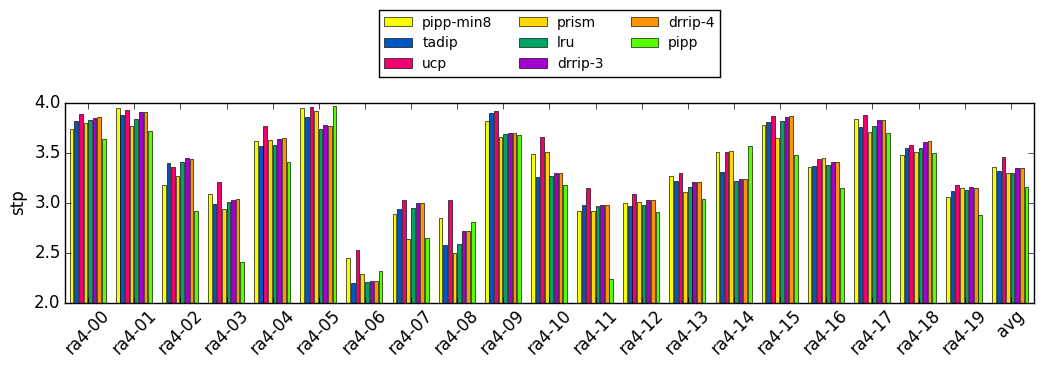
\includegraphics[width=\textwidth]{figures/results/speedup/stp-0128k-ra4}
            \caption{Random (ra4) workloads}
            \label{fig:results:4core:stp:random}
    \end{subfigure}

    \begin{subfigure}[b]{0.5\textwidth}
            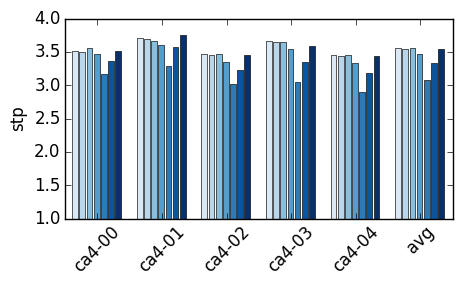
\includegraphics[width=\textwidth]{figures/results/speedup/stp-0128k-ca4}
            \caption{Cache (ca4) workloads}
            \label{fig:results:4core:stp:cache}
    \end{subfigure}%
    \begin{subfigure}[b]{0.5\textwidth}
            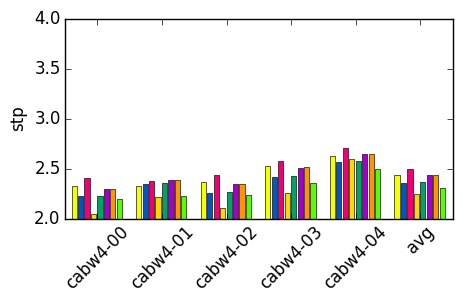
\includegraphics[width=\textwidth]{figures/results/speedup/stp-0128k-cabw4}
            \caption{Cache-Bandwidth (cabw4) workloads}
            \label{fig:results:4core:stp:cache-bw}
    \end{subfigure}

    \begin{subfigure}[b]{0.5\textwidth}
            \includegraphics[width=\textwidth]{figures/results/speedup/stp-0128k-bw4}
            \caption{Bandwidth (bw4) workloads}
            \label{fig:results:4core:stp:bw}
    \end{subfigure}%
    \begin{subfigure}[b]{0.5\textwidth}
            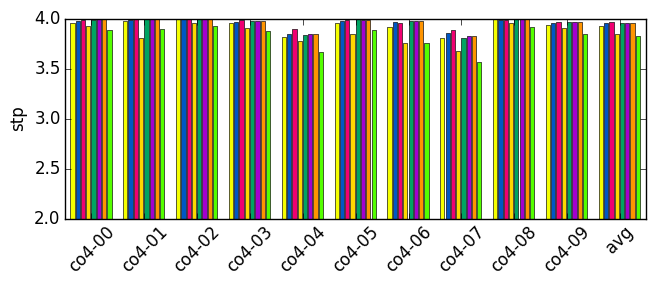
\includegraphics[width=\textwidth]{figures/results/speedup/stp-0128k-co4}
            \caption{Compute (co4) workloads}
            \label{fig:results:4core:stp:co}
    \end{subfigure}%

    \caption{4-Core workload STP results}\label{fig:results:4core:stp}
\end{figure}

\begin{figure}
    \centering
    \begin{subfigure}[b]{\textwidth}
            \includegraphics[width=\textwidth]{figures/results/speedup/hms-0128k-ra4}
            \caption{Random (ra4) workloads}
            \label{fig:results:4core:hms:random}
    \end{subfigure}

    \begin{subfigure}[b]{0.5\textwidth}
            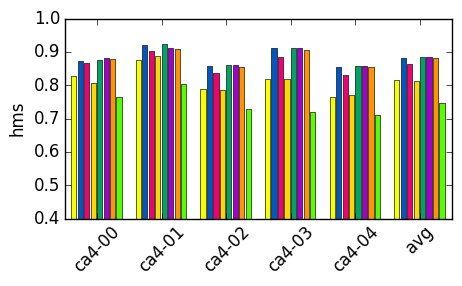
\includegraphics[width=\textwidth]{figures/results/speedup/hms-0128k-ca4}
            \caption{Cache (ca4) workloads}
            \label{fig:results:4core:hms:cache}
    \end{subfigure}%
    \begin{subfigure}[b]{0.5\textwidth}
            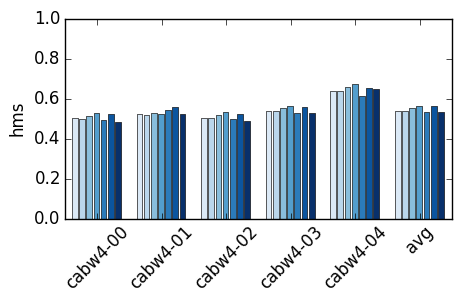
\includegraphics[width=\textwidth]{figures/results/speedup/hms-0128k-cabw4}
            \caption{Cache-Bandwidth (cabw4) workloads}
            \label{fig:results:4core:hms:cache-bw}
    \end{subfigure}

    \begin{subfigure}[b]{0.5\textwidth}
            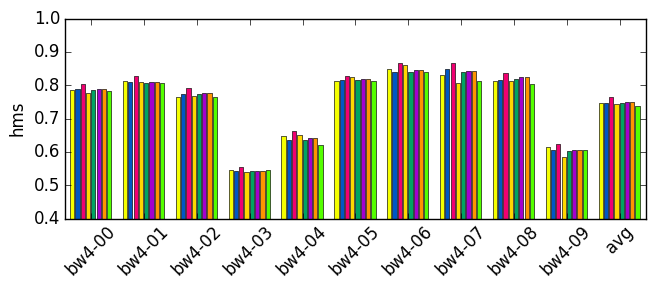
\includegraphics[width=\textwidth]{figures/results/speedup/hms-0128k-bw4}
            \caption{Bandwidth (bw4) workloads}
            \label{fig:results:4core:hms:bw}
    \end{subfigure}%
    \begin{subfigure}[b]{0.5\textwidth}
            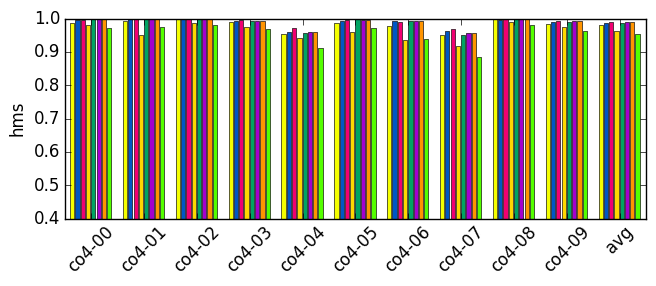
\includegraphics[width=\textwidth]{figures/results/speedup/hms-0128k-co4}
            \caption{Compute (co4) workloads}
            \label{fig:results:4core:hms:co}
    \end{subfigure}%

    \caption{4-Core workload HMS results}\label{fig:results:4core:hms}
\end{figure}

\begin{figure}
    \centering
    \begin{subfigure}[b]{\textwidth}
            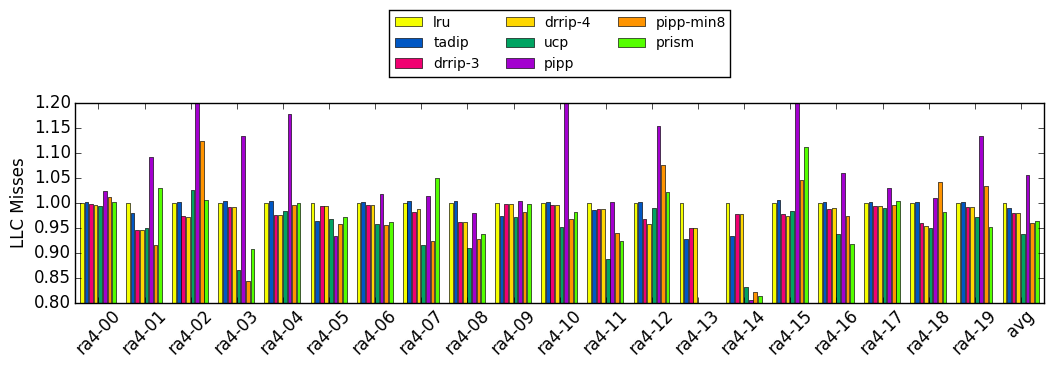
\includegraphics[width=\textwidth]{figures/results/misses/0128k-ra4}
            \caption{Random (ra4) workloads}
            \label{fig:results:4core:misses:random}
    \end{subfigure}

    \begin{subfigure}[b]{0.5\textwidth}
            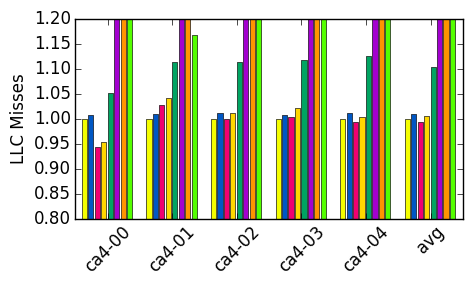
\includegraphics[width=\textwidth]{figures/results/misses/0128k-ca4}
            \caption{Cache (ca4) workloads}
            \label{fig:results:4core:misses:cache}
    \end{subfigure}%
    \begin{subfigure}[b]{0.5\textwidth}
            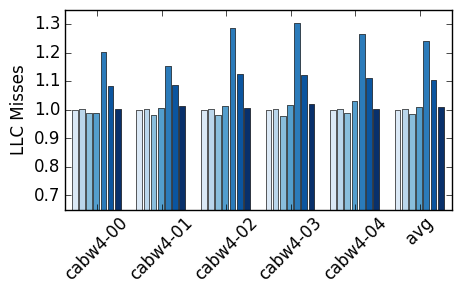
\includegraphics[width=\textwidth]{figures/results/misses/0128k-cabw4}
            \caption{Cache-Bandwidth (cabw4) workloads}
            \label{fig:results:4core:misses:cache-bw}
    \end{subfigure}

    \begin{subfigure}[b]{0.5\textwidth}
            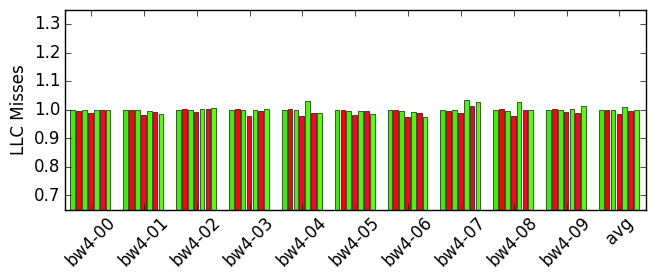
\includegraphics[width=\textwidth]{figures/results/misses/0128k-bw4}
            \caption{Bandwidth (bw4) workloads}
            \label{fig:results:4core:misses:bw}
    \end{subfigure}%
    \begin{subfigure}[b]{0.5\textwidth}
            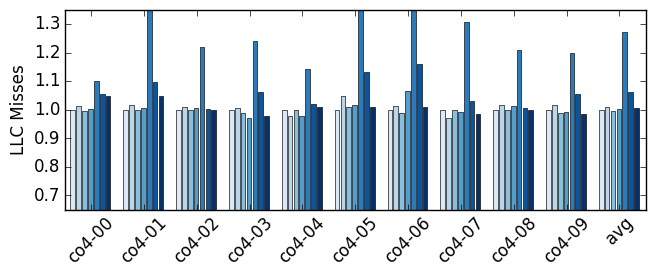
\includegraphics[width=\textwidth]{figures/results/misses/0128k-co4}
            \caption{Compute (co4) workloads}
            \label{fig:results:4core:misses:co}
    \end{subfigure}%

    \caption{4-Core workload LLC misses}\label{fig:results:4core:misses}
\end{figure}

\todo{This section is still a sketch, beware typos and incoherent reasoning}

Figure~\ref{fig:results:stp} shows the speedup of each of our 4-core workloads while figure~\ref{fig:results:misses} shows the total number of L3 misses.
For our bw workloads we expect mostly streaming and trashing access pattern, for this reason the cache partition algorithm should have little to no effect.
This assumption is confirmed when we consider the total number of L3 misses for our bandwidth bound workloads in figure~\ref{fig:results:misses:bw}.
There is little to no change between LRU, DRRIP and UCP. 
This is an expected result because they all utilize the entire cache maximizing the potential for a re-reference.
TADIP may end up running BIP for most applications. 
If this is the case, then TADIP will only utilize a small fraction of the cache, as most inserts will happen at the LRU position.
While this in theory should not affect the performance of a pure streaming or trashing access pattern, chances are there are some recency-friendly re-references TADIP misses.
PIPP also causes more misses than LRU.
We also expect that this is because there are some re-references in the access pattern. 
While the insertion policy in PIPP and LRU is expected to be the same for streaming and trashing patterns, the promotion policy differs. 
In this case, it seems that the LRU promotion policy is superior.
PIPP without streaming detection is the worst performer.
We find this reasonable as PIPP in this case on average will only use 1/4 of the cache space, limiting the potential for references.
The speedup figures for the bw workloads in figure~\ref{fig:results:stp:bw} are as expected after exploring the change is L3 misses.
We do however note that the LRU speedup is close to perfect; this could indicate that our memory bus is not saturated by our four running benchmarks.

ca workloads are built from benchmarks that are sensitive to the available cache space but not to the available bandwidth.
We expect that these have recency-friendly access patterns with small working sets compared to the LLC size.
Running a workload of all cache bound benchmarks we expect that they will begin trashing each other, resulting in four benchmarks experiencing trashing.
All algorithms in this study targets miss minimization, and they give each benchmark equal priority.
Hence we expect a small decrease in misses compared to LRU, but because of limited cache space there is still going to be trashing and reduced performance.
The miss results in figure~\ref{fig:results:misses:ca} support this expectation.
On average, DRRIP causes slightly fewer misses and TADIP and UCP slightly more misses than LRU.
We also note  that PIPP has significantly more misses than LRU.
This could be because of PIPP on average inserting in the bottom 1/4 of the LRU stack, and hence greatly lowers the chance of a reuse before replace.
PIPP without streaming detection performed close to PIPP, this is expected because ca benchmarks are not bandwidth bound and hence should not have a significant fraction of streaming accesses.
Again the speedup figures in figure~\ref{rig:results:stp:bw} show the same trend as the miss counts.

cabw workloads are expected to have a combination of streaming or trashing and recency-friendly access patterns.
Figure~\ref{fig:results:misses:cabw} shows the miss counts for these workloads. 
These results are in many ways a combination of the bw and ca result. 
With most algorithms performing as LRU and PIPP showing a increase in misses.
The increase of PIPP is not as large in the ca workloads.
we expect this is because this increase comes from execution phases where all or most of the benchmarks are recency-friendly and are trashing each other.
In phases where benchmarks are streaming the difference between PIPP and the others is smaller as shown by our bw workloads.
The speedup of our cabw workloads shows an interesting effect.
Even if UCP on average causes more misses than LRU it results in an average speedup.
\todo{explain why, most likely because of the block \'protection\' given by UCP}

Compute. PIPP underperforms again but has little effect on speedup as they are not bounded by the memory system. Close to perfect speedup for all algorithms.

\todo{Once Stallo run completes include random workloads as well. We should see clear differences here because we will have various access patterns, not four benchmarks with the same type of pattern}